\documentclass[titlepage,12pt,oneside,a4paper]{article}

% packages
\usepackage{times}         % font
\usepackage{geometry}      % set margins
\usepackage{listings}      % for code listings
\usepackage{graphicx}      % for inserting images
\usepackage{multicol}      % for multi columns pages
\usepackage{rotating}
% turn on page numbers and section name on each page
\pagestyle{headings}

\graphicspath{{images/}}     % define the images directory

% define the formatting for inline code snippets
\newcommand{\code}[1]{{\texttt{#1}}}

% no paragraph indentation
\setlength{\parindent}{0em}

% one line between each paragraph
\setlength{\parskip}{1em}

% Title Page
\title{MIPS PIPELINED PROCESSOR}
\author{
	Abdelrahman Mohamed Abdelnabi\\
	3466
	\and
	Ahmed Lotfey Atia Siam \\
	4129
	\and
	Ahmed Mohamed Fayez \\
	4130
}

%=====================================%
% DOCUMENT
%=====================================%
\begin{document}
\maketitle

\begin{abstract}
	Pipelining is a powerful way to improve the	throughput of a digital system. We design a pipelined processor by subdividing the single-cycle processor into five pipeline stages. Thus, five instructions can execute simultaneously, one in each stage. Because each stage has only one-fifth of the entire logic, the clock frequency is almost five times faster. Hence, the latency of each instruction is ideally unchanged, but the throughput is ideally five times better. Microprocessors execute millions or billions of instructions per second, so throughput is more important than latency. Pipelining introduces some overhead, so the throughput will not be quite as high as we might ideally desire, but pipelining nevertheless gives such great advantage for so little cost that all modern high-performance microprocessors are pipelined. In this Lab, we will design and implement a MIPS piplined  processor using\textit{ System Verilog}.
\end{abstract}

%=====================================%
% CHAPTER 1
%=====================================%


\section{Introduction}
This is a 5 stage (Fetch, Decode, Execute, Memory, Write Back) MIPS pipelined processor.

To ease the modification process and allow readers to see how we went on to modify the source code to implement a new instruction, we use \textit{git} as a \textit{version control system}. After most of the instructions, there will be a command that you can run, after \textit{cloning the project from git}, to see the changes that we made at each step.

You can clone the project using this command:\\
\code{git clone https://github.com/abdelrahmanabdelnabi/\\MIPS-Pipelined-Processor.git}

alternatively, if you don't have git, you can to this link to see the project through its stages (i.e \textit{commits}) on \textit{Github}:\\
\code{https://github.com/abdelrahmanabdelnabi/MIPS-Pipelined-Processor}

\subsection{Supported Instructions}
\label{ISA}
	\begin{center}
		
		\begin{tabular}{| c | c | c |}
			\hline
			% TODO: add table of supported instructions here
			Opcodes &Example Assembly& Semantics\\
			\hline
			add &add \$1, \$2, \$3 &\$1 = 2 + \$3\\
			\hline
			sub &sub \$1, \$2, \$3 &\$1 = 2 - \$3\\
			\hline
			add immediate &addi 1, \$2, 100 &\$1 = 2 + 100\\
			\hline
			multiply &mult 2, \$3 &hi, lo = \$2 * \$3\\
			\hline
			divide &div \$2, \$3 &lo = 2/\$3, hi = \$2 mod \$3\\
			\hline
			move from hi& mfhi \$1 &\$1 = hi\\
			\hline
			move from low& mflo \$1 &\$1 = lo\\
			\hline
			and &and \$1, \$2, \$3& \$1 = \$2 \& \$3\\
			\hline
			or &or \$1, \$2, \$3& \$1 = \$2 $|$ \$3\\
			\hline
			shift left logical &sll \$1, \$2, 10&\$1 = \$2 $<<$ 10\\
			\hline
			shift right logical & srl \$1, \$2, 10 &\$1 = \$2 $>>$ 10\\
			\hline
			load word &lw \$1, \$2(100) &\$1 = ReadMem32(\$2 + 100)\\
			\hline
			store word &sw \$1, \$2(100)& WriteMem32(\$2 + 100, \$1)\\
			\hline
			load byte &lb \$1, \$2(100)& \$1 = SignExt(ReadMem8(\$2 + 100))\\
			\hline
			store byte &sb \$1, \$2(100)& WriteMem8(\$2 + 100, \$1)\\
			\hline
			branch on equal &beq \$1, \$2, Label &if (\$1 == \$2) goto Label\\
			\hline
			branch on not equal &bne \$1, \$2, Label &if (\$1 != \$2) goto Label\\
			\hline
			set on less than &slt \$1, \$2, \$3 &if (\$2 $<$ \$3) \$1 = 1 else \$1 = 0\\
			\hline
			set on less than immediate& slti \$1, \$2, 100 &if (\$2 $<$ 100) \$1 = 1 else \$1 = 0\\
			\hline
			jump &j Label &goto Label\\
			\hline
			jump register &jr \$31 &goto \$31\\
			\hline
			jump and link & jal Label&\$31 = PC + 4; goto Label\\
			\hline
		\end{tabular}
	\end{center}
\subsection{Initial Version}
We will use the MIPS pipelined version developed in our textbook as the initial version which we will build on it other components to support the remaining instructions.

This version already supports the instructions:add (\code{add}), sub (\code{sub}), add immediate (\code{addi}), and (\code{and}), or (\code{or}), load word (\code{lw}), sw (\code{sw}), branch on equal (\code{beq}), set on less than (\code{slt}), jump (\code{j}), with a hazard and control unit.

The initial version also uses early branch resolution to make a branch decision in the decode stage.

\subsection{fixing a small error}

The version in the textbook uses an equal comparator in the decode stage for early branch resolution. The datapath module instantiates an \code{eqcmp} object which is not defined in any file. we implemented the module ourselves. You can find the source code of the module in appendix \ref{appendix:src:mipsparts}

The pipelined processor writes the register file in the first half of the write-back stage and reads it the second half of the decode stage. However, this was not the case in the text book code. The register file was written and read at the same time. To fix this, we added a delay of 5 time units after the write.

After this two fixes the test bench indicates a successful simulation.
%=====================================%
% CHAPTER 2
%=====================================%

\section{Extending the Design}

In this section we will modify and/or extend the design of the MIPS pipelined processor to support new instructions as indicated in section \ref{ISA}

\subsection{Branch on Not Equal}
supporting this instruction is relatively easy, as branch on equal is already supported. We just have to detect the not equal condition. To do this, we modify the control unit to detect the opcode of \code{bne} and generate the required control signals.

We add a new control signal, \code{bneD} which is 1 when the instruction in the decode stage is a \code{bne}. all the control signals for \code{beq} and \code{bne} are same except for the signals \code{branchD} and \code{bneD}, their values are reversed. 

The logic for \code{pcsrcD} is now different. \code{prcsrcD} is now 1 when either of the conditions of \code{beq} and \code{bne} are satisfied. i.e \code{pcsrcD = (branchD \& equalD) | (bneD \& $\sim$equalD)}


The logic for stalling will need to detect the \code{bne} instruction and stall as necessary exactly the same like for \code{beq}. Therefore the hazard unit takes a new input which the control signal \code{bneD}.

This completes all the necessary changes required for the control unit and datapath. Figure \ref{fig:bne} shows all the changes made to the data path.

\begin{figure}
	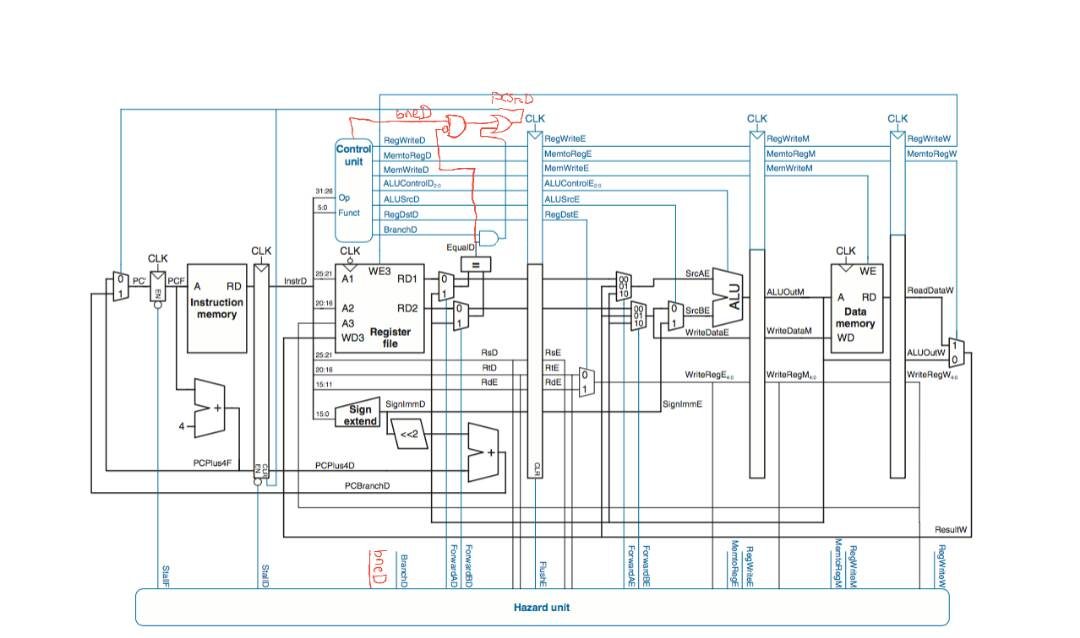
\includegraphics[width=\textwidth]{bne.jpeg}
	\centering
	\caption{Pipelined processor with support for \code{bne}}
	\label{fig:bne}
\end{figure}

We test the instruction by adding a \code{bne \$s2, \$2, 0x30} after the first instruction of our test program. Testing shows that the stall and branching works properly both when the branch is taken and not taken.

To see the changes to the source code to support this instruction run:\\
\code{git diff abdc c7c0}

\subsection{load byte}

An example of this instruction is \code{lb \$s1, 40(\$s0)}, which loads the byte at the address of 40 + reg(\$s0), sign-extends it and puts it in register \$s1.

To support this instruction we need to select a byte out of the 4 bytes read from memory each cycle according to $memaddr_{[1:0]}$, and then sign extend it to 32 bits. We will need a control signal that tells us that this is a \code{lb} instruction, then at the memory stage, we will select either the 32 bits memory output or the sign extended byte according to this signal. This implies using a 2-1 multiplexer that has this control signal as its selector. We will need another multiplexer to select the proper byte from the memory word read. Figure \ref{fig:lb} shows the modifications made to the data path.

\begin{figure}
	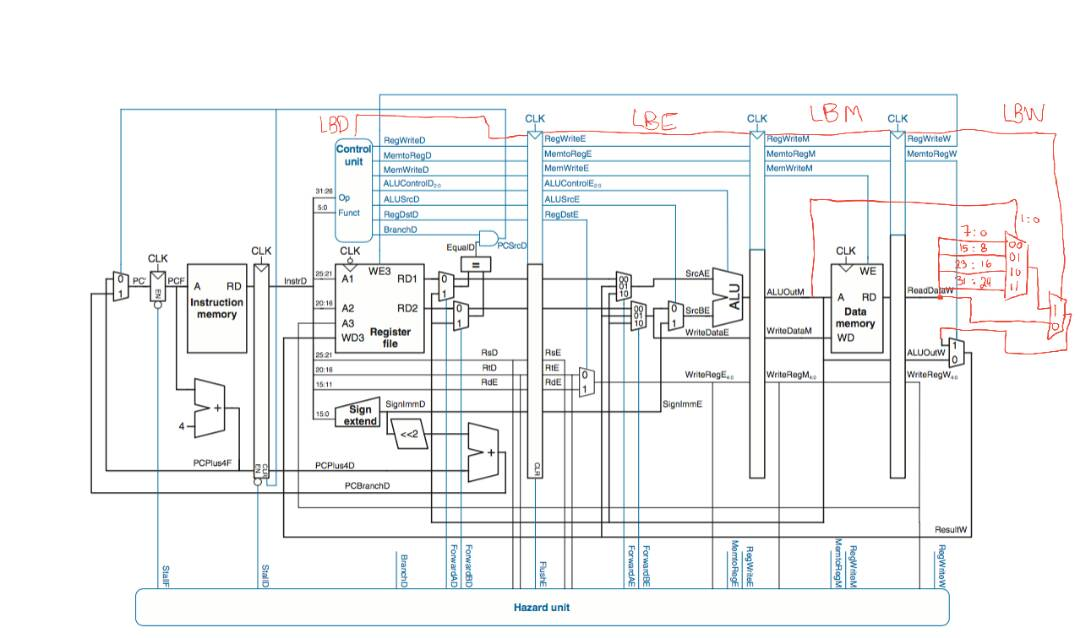
\includegraphics[width=\textwidth]{lb.jpeg}
	\centering
	\caption{Pipelined processor with support for \code{lb}}
	\label{fig:lb}
\end{figure}

We test the instruction by modifying our test program to use \code{lb} instead of \code{lw} (temporarily). Since this should still the load 7 into register \$s2, it won't modify the final result. We run the simulation and it indicates successful completion. we also see that the \code{lbW} signal takes the value 1 only at the write-back stage of the load byte instruction.

To see the changes made to the code to support this instruction run:\\
\code{git diff 18dc 5547}

\subsection{Logical Shift}

logical shift left, \code{sll} and right \code{srl} are R-Type instructions. The infrastructure for R-Type instructions already exists and therefore no significant changes to the datapath are required. Most of the change occurs because of the \textit{shamt} field needs to be passed to the execute stage and the ALU. We add the shamt to the execute stage pipeline register, and modify the ALU to accept it as an input. The ALU decoder will need to detect the shift instructions and generate the proper ALUcontrol signals, so we add 2 rows to the decoder's truth table, one for each instruction. Moreover we extend the ALUControl signal to 4 bits to be able to encode the two new instructions. Table \ref{table:aluctrl} shows new the ALU control signals truth table.

To test the two new instructions, we add \code{sll \$s2, \$s2, 4} and \code{srl \$s2, \$s2, 4} just before the last instruction in out test program. This won't modify the final result since \$s2 contains 7 before running the shift instructions and we shift left then right by the same amount. Running the simulation, the correct result is written and completes successfully.

To see the changes made to the code to support these instructions run:\\
\code{git diff 2656 5ab4} 
\begin{table}
\begin{center}
	
	\begin{tabular}{|c|c|}
		\hline
		$ALUControl_{3:0}$ & Function \\
		\hline
		0000 & A AND B \\
		0001 & A OR B \\
		0010 & A + B \\
		0011 & not used \\
		1000 & A AND $\overline{B}$ \\
		1001 & A OR $\overline{B}$ \\
		1010 & A - B \\
		1011 & SLT \\
		0100 & B $<<$ shamt \\
		0101 & B $>>$ shamt \\
		\hline
	\end{tabular}
\end{center}
	\caption{ALU control truth table}
	\label{table:aluctrl}
\end{table}


\subsection{Jump and Link}
The semantics of \code{jal label} is \code{\$ra = PC + 4, goto label}. \code{jal} does exactly the same as jump but writes the value of PC onto register 31, the return address register.

Implementing this instruction won't affect the hardware as much because \code{jal} is mixture of jump and R-Type, both of which are already supported. We will add to the datapath a new mux that selects which data to write to the register file. The new mux will choose between \textit{ResultW} and \textit{PCPlus4W}, according to the selector \textit{jal}, which is a new control signal that is true only if the instruction is \code{jal}. The \textit{PCPlus4} signal must be passed from the decode to the write back stage so that we can write it to the register file. We will also extend the \textit{RegDst} mux, which selects which register to write on, to accept the number 31 as a new input. This means that we need to extend the mux selector control signal, \textit{RegDst}, to 2 bits.

The main decoder sets the \textit{Jump} signal to 1 so that the hazard unit handles flushes appropriately. Also no modifications to the hazard unit are required since the writing to register file part of the instruction (\textit{WriteRegE} and \textit{RegWriteE} signals) is the same as for R-Type instructions. Figure \ref{fig:jal} shows the modifications made to the data path.

\begin{figure}
	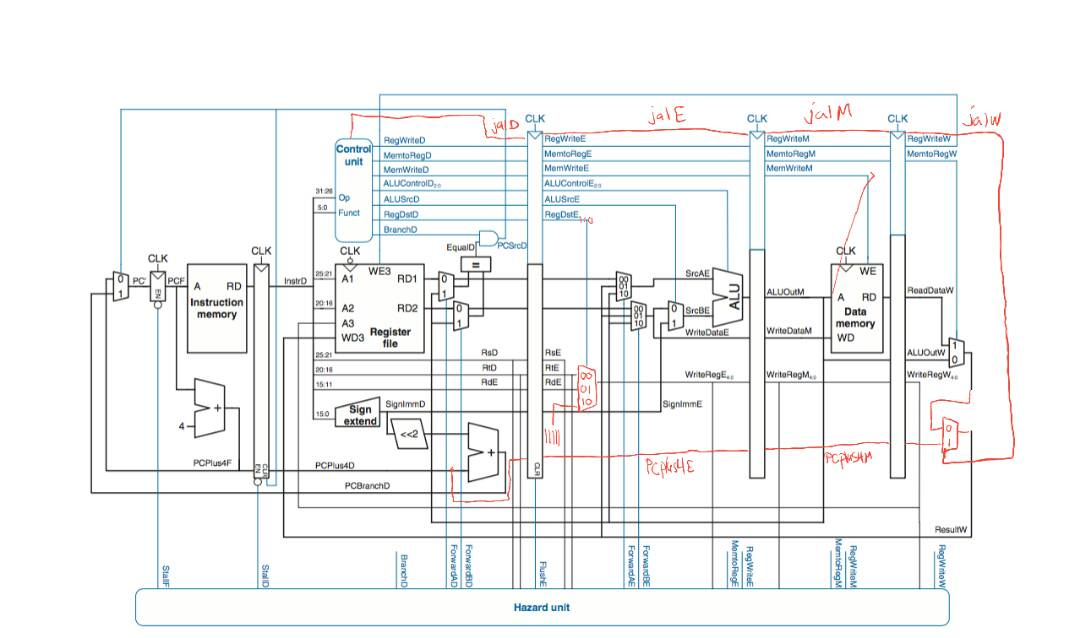
\includegraphics[width=\textwidth]{jal.jpeg}
	\centering
	\caption{Pipelined processor with support for \code{jal}}
	\label{fig:jal}
\end{figure}

To test the instruction, we modify the test program to use \code{jal} instead of \code{j} on the instruction at address 3C. This won't change the results. It will only write the value of PC + 4, which is 40 at the time of executing the instruction, to the return address register, \$ra.

Figure \ref{fig:jaltest} shows the simulation of the test program with \code{jal} being used. Notice the simulation ends successfully the \textit{jalD} and \textit{jalW} signals are 1 when the instruction is decoded and when the result is written to the register file. Also notice that the return address register has the correct value (0x40) written to it, at the second half of the write back stage of the \code{jal} instruction.

To see the changes made to the code to support this instruction run: \\
\code{git diff 8f6f e0ea -- mips.sv controller.sv datapath.sv \\ maindecoder.sv}

\begin{figure}
	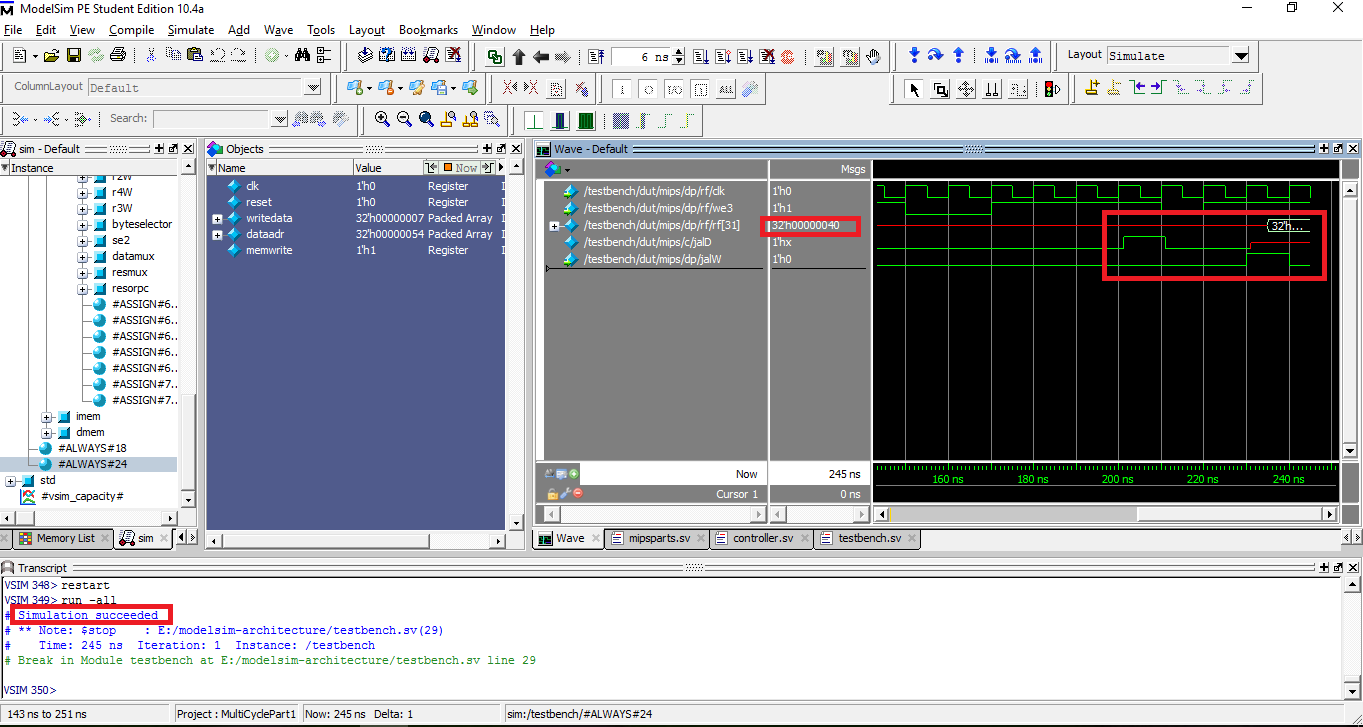
\includegraphics[width=\textwidth]{jaltest.png}
	\centering
	\caption{simulation and testing of \code{jal}}
	\label{fig:jaltest}
\end{figure}

\subsection{Multiplication and Division}
As the textbook states, Multiplication and division are somewhat different from other arithmetic operations. Multiplying two 32-bit numbers produces a 64-bit product. Dividing two 32-bit numbers produces a 32-bit quotient and a 32-bit remainder.

The MIPS architecture has two special-purpose registers, hi and lo, which are used to hold the results of multiplication and division. \code{mult \$s0, \$s1} multiplies the values in \$s0 and \$s1. The 32 most significant bits of the product are placed in hi and the 32 least significant bits are placed in lo. Similarly, \code{div \$s0, \$s1} computes \$s0/\$s1. The quotient is placed in lo and the remainder is placed in hi.

\subsubsection{The Multiplication and Divison unit}
The normal ALU doesn't support multiplication and division operations. In reality, multiplication and division are executed using dedicated expensive circuits and usually take several clock cycles to finish. Our Design will be simple however. We will add a new unit that operates in the execute stage alongside the ALU to carry out multiplication and division.

The unit's inputs are the two numbers, which are exactly the same as those provided to the ALU, and a flag that tells the unit to either multiply or divide. The outputs are two 32-bit numbers, the hi and lo values. Appendix \ref{appendix:multdivunit} shows the unit's code.

\subsubsection{Hi and Lo Registers}
The hi and lo registers are used to support 64-bit multiplication and divsion results. They exist outside the register file as separate registers. However, we write them in the first half of the write back cycle and read them in the second half of the decode cycle. The registers are encapsulated in module with a write enable signal. It has two input ports to input the data to be written, and two output ports that has the data read.

\subsubsection{Supporting \code{Mult} and \code{div} Instructions}
Once we add the multiplication and division unit and the hi and lo registers to the datapath, it's only the addition or few control signals that's remaining. We add two new control signals, \textit{multordiv} and \textit{hlwrite}, the former tells the unit to multiply or divide, and the latter tells the hi and lo module to write the data at its input port to the registers. The control signals and the result of multiplication unit will be passed through the pipeline registers to the write back stage as usual (except for \textit{multordiv} which is needed only in the execute stage).

Two more rows are added to the main decoder to detect \code{mult} and \code{div} and generate the needed control signals.

\subsubsection{Supporting \code{mfhi} and \code{mflo}}
\label{mfhl}
\code{mfhi} and \code{mflo} turn out to be simple to implement as they operate in the write back stage only. The data needed, i.e the hi or lo values, are only needed in the write back stage, which eliminates the need for RAW hazard handling as no forwarding or stalling is needed.

To implement this instruction we need to select which value to write to the register file. We add a new mux that has the \textit{ResultW}, hi, and lo as its inputs. The inputs are selected according to the instruction in execution, whether it's a \code{mfhi}, \code{mflo}, or any other instruction. Therefore we will need a 2 bit control signal, \textit{mvhl}, for the multiplexer selectors.

Figure \ref{fig:mdhl} shows all the modifications made to the data path to support \code{mult}, \code{div}, \code{mvhi}, and \code{mflo}.

\begin{figure}
	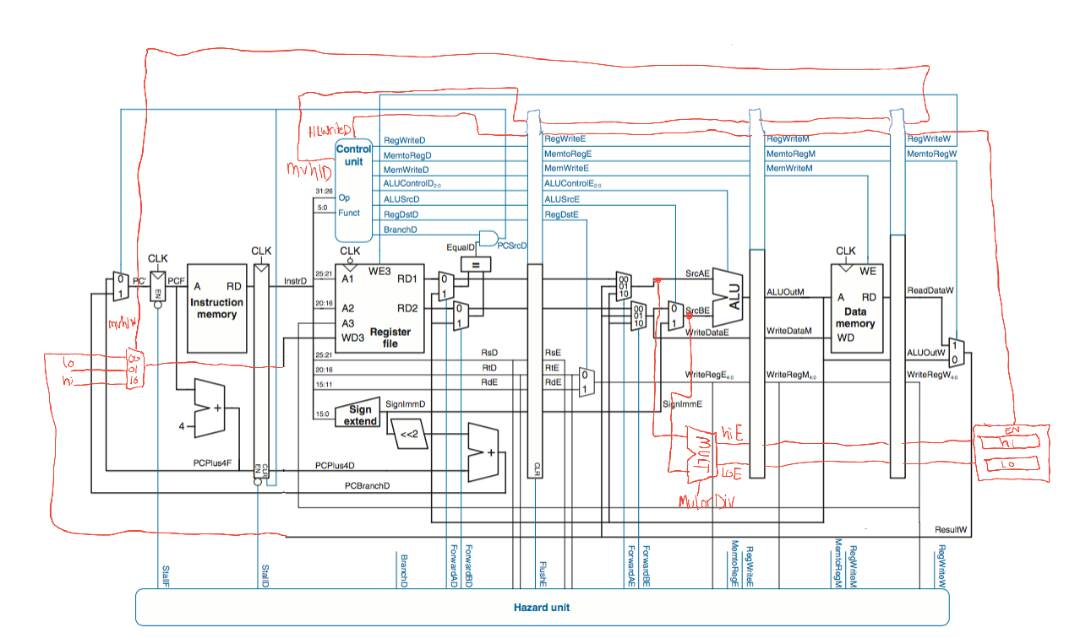
\includegraphics[width=\textwidth]{mdhl.jpeg}
	\centering
	\caption{Pipelined processor with support for \code{mult}, \code{div}, \code{mvhi}, and \code{mflo}}
	\label{fig:mdhl}
\end{figure}
 To see the changes made to the source code to support these instructions, run:\footnote{we forgot to add the \textit{hiandlo } module to git at this commit, however you can still view the module starting from commit number \code{4503}}\\
 \code{git diff 2dce 306f} 

\subsubsection{Hazard Handling}
For \code{mult} and \code{div}, the operands for the instructions are properly already handled by the hazard unit since the forwarded operand is the one that the multiplication unit uses. For \code{mfhi} and \code{mflo}, the operands, i.e the hi and lo registers, are read at the memory cycle which guarantees that the proper value is read, as indicated in section \ref{mfhl}.

\subsection{Set If Less than Immediate}
The ALU already supports \code{slt}, we just need to pass the immediate field as the second operand to the ALU. The datapath already has a path for passing the sign-extended immediate to the ALU, by setting \textit{ALUSrc} to 1. We assign the \textit{ALUOp} 11 to subtract B from A and set the result to 1 if A \textless{ } B and 0 otherwise. Table \ref{table:aluop} shows the new ALUOp table.

\begin{table}
	\begin{center}
		\begin{tabular}{|c|c|}
			\hline
			$ALUOp_{1:0}$ & Operation \\
			\hline
			00 & Add \\
			01 & Sub \\
			10 & Look at \textit{funct} \\
			11 & SLT \\
			\hline
		\end{tabular}
	\end{center}
	\caption{ALU operation Table}
	\label{table:aluop}
\end{table}

\subsection{Jump Register}
\code{jr} jumps to the address stored in \textit{reg(rs)}, instead of the JTA calculated from the immediate field of a jump instruction. Unlike the normal jump, \code{jr} is an R-Type instruction.

To Implement \code{jr}, we will extend the mux that selects which data gets written on the PC register. The extended mux will choose between PC’ (the result of the previous mux), jump target address, and SrcAD (value of \textit{reg(rs)}). We added a new control signal, \textit{jr} that is true only if the instruction is \code{jr}. Now concerning the Selector of the extended mux , we will use the jump control signal as the least significant bit of the selector and the new \textit{jr} control signal as the most significant bit. And of course the proper value of the selectors are generated by the main decoder. Figure \ref{fig:jr} shows the modifications to the data path to implement this instruction.

\begin{figure}
	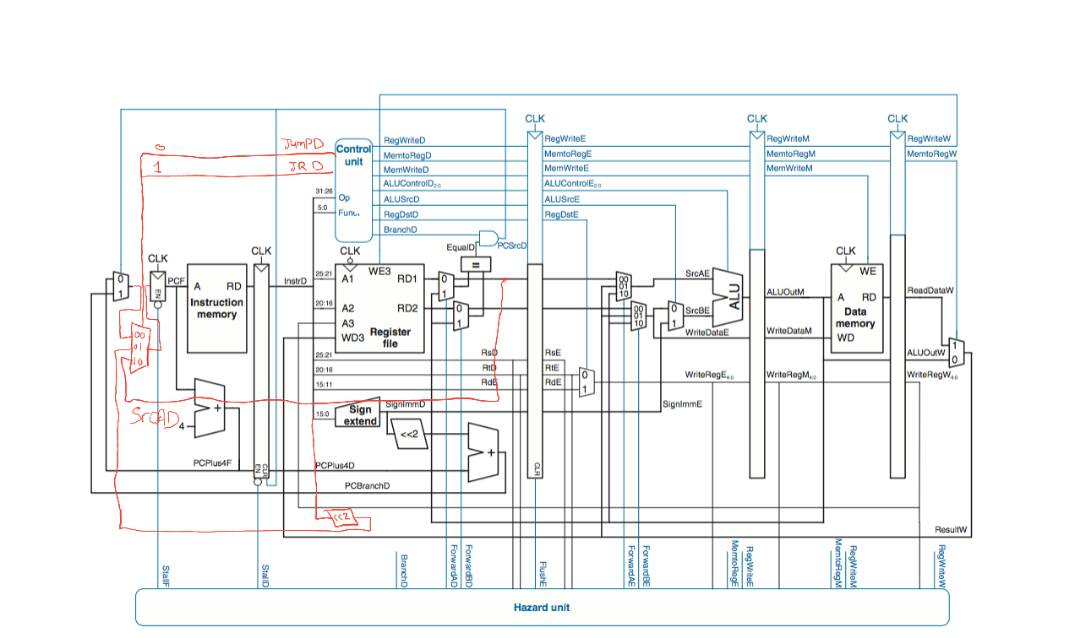
\includegraphics[width=\textwidth]{jr.jpeg}
	\centering
	\caption{Pipelined processor with support for \code{jr}}
	\label{fig:jr}
\end{figure}

\subsection{Store Byte}
According to the textbook and the final project description, store byte stores the least significant bits of a register in a byte in memory without affecting the remaining bytes in the same word in memory. This requires modifying the memory to able to write only one byte.

We add a pin to the memory that specifies if the memory should store only one byte of the data at its input port. The pin is connected to \textit{sb}, a new control signal. Appendix \ref{appendix:dmem} has the modified source code for the memory module. Other than that, no more modifications are required. No changes are made to the data path.

To see the source code modifications made to support this instruction run:\\
\code{ git diff b26a ea0a}

\section{Final Main Decoder Table}
\begin{center}
\begin{tabular}{|c|c|c|c|c|c|c|c|c|c|c|c|c|c|c|c|c|c|}
	\hline
\begin{turn}{-90}Inst\end{turn}&\begin{turn}{-90}Opcode\end{turn}&\begin{turn}{-90}RegWrite\end{turn}&\begin{turn}{-90}RegDst\end{turn}&\begin{turn}{-90}ALUSrc\end{turn}&\begin{turn}{-90}Branch\end{turn}&\begin{turn}{-90}Bne\end{turn}&\begin{turn}{-90}MemWrite\end{turn}&\begin{turn}{-90}MemtoReg\end{turn}&\begin{turn}{-90}Jump\end{turn}&\begin{turn}{-90}Jal\end{turn}&\begin{turn}{-90}Jr\end{turn}&\begin{turn}{-90}Lb\end{turn}&\begin{turn}{-90}Sb\end{turn}&\begin{turn}{-90}MultorDiv\end{turn}&\begin{turn}{-90}hlwrite\end{turn}&\begin{turn}{-90}mvhl\end{turn}&\begin{turn}{-90}ALUOp\end{turn}\\
\hline
R-Type & 000000 & 1 & 00 & 0 & 0 & 0 & 0 & 0 & 0 & 0 & 0 & 0 & 0 & 0 & 0 & 00 & 00 \\
\hline
JR & 000000 & 0 & 00 & 0 & 0 & 0 & 0 & 0 & 0 & 0 & 1 & 0 & 0 & 0 & 0 & 00 & 00 \\
\hline
MULT & 000000 & 0 & 00 & 0 & 0 & 0 & 0 & 0 & 0 & 0 & 0 & 0 & 0 & 1 & 1 & 00 & 00 \\
\hline
DIV & 000000 & 0 & 00 & 0 & 0 & 0 & 0 & 0 & 0 & 0 & 0 & 0 & 0 & 0 & 1 & 00 & 00 \\
\hline
MFLO & 000000 & 1 & 01 & 0 & 0 & 0 & 0 & 0 & 0 & 0 & 0 & 0 & 0 & 0 & 0 & 01 & 00 \\
\hline
MFHI & 000000 & 1 & 01 & 0 & 0 & 0 & 0 & 0 & 0 & 0 & 0 & 0 & 0 & 0 & 0 & 10 & 00 \\
\hline
LW & 100011 & 1 & 00 & 1 & 0 & 0 & 0 & 1 & 0 & 0 & 0 & 0 & 0 & 0 & 0 & 00 & 00 \\
\hline
SW & 101011 & 0 & 00 & 1 & 0 & 0 & 1 & 0 & 0 & 0 & 0 & 0 & 0 & 0 & 0 & 00 & 00 \\
\hline
BEQ & 000100 & 0 & 00 & 0 & 1 & 0 & 0 & 0 & 0 & 0 & 0 & 0 & 0 & 0 & 0 & 00 & 01 \\
\hline
BNE & 000101 & 0 & 00 & 0 & 0 & 1 & 0 & 0 & 0 & 0 & 0 & 0 & 0 & 0 & 0 & 00 & 01 \\
\hline
ADDI & 001000 & 1 & 00 & 1 & 0 & 0 & 0 & 0 & 0 & 0 & 0 & 0 & 0 & 0 & 0 & 00 & 00 \\
\hline
J & 000010 & 0 & 00 & 0 & 0 & 0 & 0 & 0 & 1 & 0 & 0 & 0 & 0 & 0 & 0 & 00 & 00 \\
\hline
LB & 100000 & 1 & 00 & 1 & 0 & 0 & 0 & 1 & 0 & 0 & 0 & 1 & 0 & 0 & 0 & 00 & 00 \\
\hline
SB & 101000 & 0 & 00 & 1 & 0 & 0 & 1 & 0 & 0 & 0 & 0 & 0 & 1 & 0 & 0 & 00 & 00 \\
\hline
JAL & 000011 & 1 & 10 & 0 & 0 & 0 & 0 & 0 & 1 & 1 & 0 & 0 & 0 & 0 & 0 & 00 & 00 \\
\hline
SLTI & 001010 & 1 & 00 & 1 & 0 & 0 & 0 & 0 & 0 & 0 & 0 & 0 & 0 & 0 & 0 & 00 & 11 \\
\hline

\end{tabular}
\end{center}

\section{Simulation and Testing}
To ensure that our modifications have been completed correctly and work together as intended, we test the completed pipelined processor on 3 programs, listed in appendix \ref{appendix:tests}.

Because there are too many signals to show and the program takes from 250 to 950 ns to execute, it would be cumbersome to include the simulation screenshots here as they it would take a lot of screenshots to show the simulation of one program. Therefore, its better if you could download the source files attached with this report, compile and run them and view the results on you screen. All the 3 programs have been tested and all show correct results.

%=====================================%
% Source Code appendix
%=====================================%
\newpage
\appendix
\begin{multicols}{2}

\section{Source Code}
\label{appendix:src}
\subsection{datapath.sv}
\lstinputlisting[breaklines=true,basicstyle=\tiny,language=verilog]{../datapath.sv}

\subsection{maindecoder.sv}
\lstinputlisting[breaklines=true,basicstyle=\tiny,language=verilog]{../maindecoder.sv}

\subsection{aludecoder.sv}
\lstinputlisting[breaklines=true,basicstyle=\tiny,language=verilog]{../aludecoder.sv}

\subsection{controller.sv}
\lstinputlisting[breaklines=true,basicstyle=\tiny,language=verilog]{../controller.sv}

\subsection{multdivunit.sv}
\label{appendix:multdivunit}
\lstinputlisting[breaklines=true,basicstyle=\tiny,language=verilog]{../multdivunit.sv}

\subsection{hiandlo.sv}
\lstinputlisting[breaklines=true,basicstyle=\tiny,language=verilog]{../hiandlo.sv}

\subsection{alu.sv}
\lstinputlisting[breaklines=true,basicstyle=\tiny,language=verilog]{../alu.sv}

\subsection{mipsmem.sv}
\label{appendix:dmem}
\lstinputlisting[breaklines=true,basicstyle=\tiny,language=verilog]{../mipsmem.sv}

\subsection{mips.sv}
\lstinputlisting[breaklines=true,basicstyle=\tiny,language=verilog]{../mips.sv}

\subsection{topmulti.sv}
\lstinputlisting[breaklines=true,basicstyle=\tiny,language=verilog]{../topmulti.sv}

\subsection{hazard.sv}
\lstinputlisting[breaklines=true,basicstyle=\tiny,language=verilog]{../hazard.sv}

\subsection{testbench.sv}
\label{appendix:src:mipsparts}
\lstinputlisting[breaklines=true,basicstyle=\tiny,language=verilog]{../testbench.sv}

\section{Test Programs}
\label{appendix:tests}

\subsection{Textbook Test Program}
stores 7 in memory location 84.

\code{main: addi \$2, \$0, 5\\
	addi \$3, \$0, 12\\
	addi \$7, \$3, −9\\
	or \$4, \$7, \$2 \\
	and \$5, \$3, \$4\\
	add \$5, \$5, \$4\\
	beq \$5, \$7, end\\
	slt \$4, \$3, \$4\\
	beq \$4, \$0, around\\
	addi \$5, \$0, 0\\
	around: slt \$4, \$7, \$2\\
	add \$7, \$4, \$5\\
	sub \$7, \$7, \$2\\
	sw \$7, 68(\$3)\\
	lw \$2, 80(\$0)\\
	j end\\
	addi \$2, \$0, 1\\
	end: sw \$2, 84(\$0)}\\

\subsection{Series Sum}
Adds the numbers from 1 to 10 inclusive.

\code{main:
	addi \$7, \$0, 10 \\
	add \$a0, \$0, \$7\\
	jal seriesSum\\
	sw \$v0, 84(\$0)\\
	seriesSum:\\
	add \$v0, \$0, \$0\\
	loop:\\
	add \$v0, \$v0, \$a0\\
	addi \$a0, \$a0, -1\\
	bne \$0, \$a0, loop\\
	jr \$ra\\} 

\subsection{Recursive Factorial}
calculates the factorial of a number, in this test the number is 5.

\code{addi \$sp, \$0, 400 \\
	main:
	addi \$a0, \$0, 5\\
	jal factorial\\
	add \$s0, \$v0, \$0\\
	sw \$s0, 84(\$0)\\
	factorial: addi \$sp, \$sp, -8\\
	sw \$a0, 4(\$sp)\\
	sw \$ra, 0(\$sp)\\
	addi \$t0, \$0, 2\\
	slt \$t0, \$a0, \$t0
	beq \$t0, \$0, else\\
	addi \$v0, \$0, 1\\
	addi \$sp, \$sp, 8\\
	jr \$ra\\
	else: addi \$a0, \$a0, -1\\
	jal factorial\\
	lw \$ra, 0(\$sp)\\
	lw \$a0, 4(\$sp)\\
	addi \$sp, \$sp, 8\\
	mult \$a0, \$v0\\
	mflo \$v0\\
	jr \$ra\\}

\end{multicols}
\end{document}          
